\subsection{Volume of Particular Tori by Exhaustion}

In this section we look at using a method of exhaustion/rearrangement to evaluate a torus created from rotating
a 2-dimensional cross-section that has a vertical line of symmetry. 

\subsubsection*{The Setup}

The volume of a solid of revolution is provided by the classic Pappus' Centroid Theorem. The
theorem is mainly attributed to Pappus of Alexandria and Paul Guldin. Now, Pappus is a
mathematician of ancient Greece, and Guldin wrote his manuscript containing the theorem,
\textit{De centro gravitatis trium specierum quanitatis continuae} in 1640 (two years before
Newton was born). Typically this theorem is presented using integral calculus. However, given
that the creators of the theorem predate the invention of integral calculus, we are lead to wonder
if we can prove the theorem more directly using a method of exhaustion.

Here we will prove the theorem in the case that the cross-section of the revolution has a vertical
line of symmetry, much like in the figure below.

\begin{figure}[h]
\centering
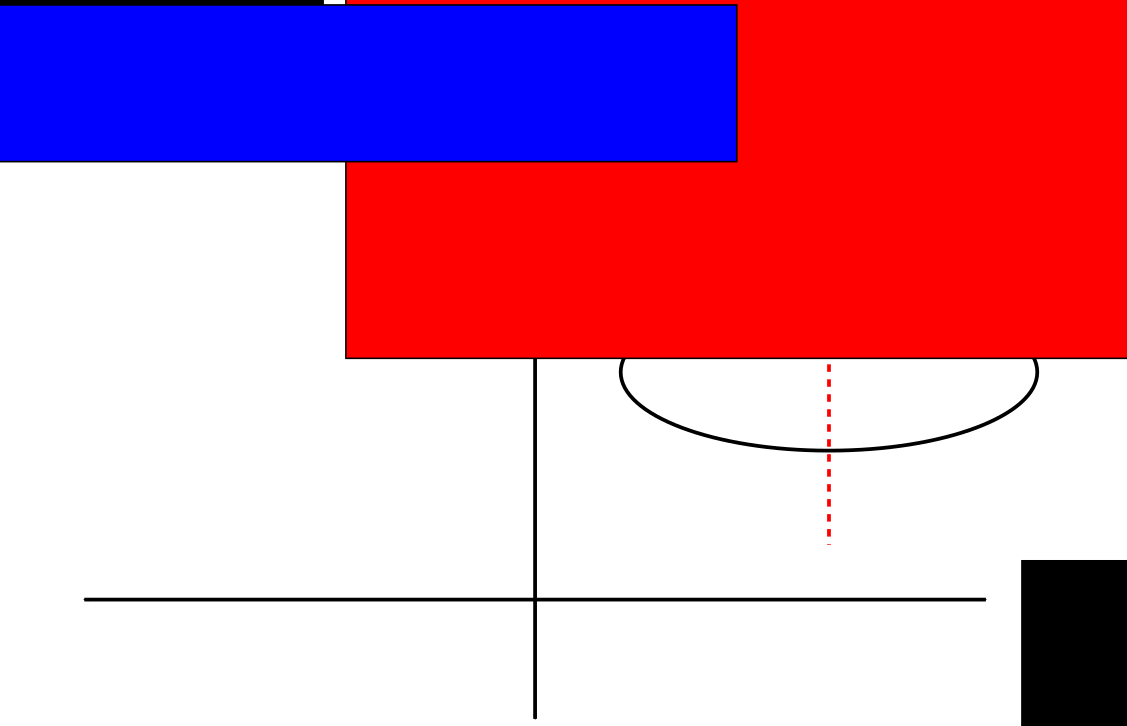
\includegraphics[width = 0.7 \textwidth]{_generated/pappus_cross_section.pdf}
\end{figure}

\subsubsection*{The Problem}

Given that the cross-section of the body of revolution has a vertical line of symmetry, find a
method of exhaustion/rearrangement that will compute its volume.

\subsubsection*{The Solution}

We divide the body of revolution into \(4n\) pieces by the angle of revolution, i.e. a number of 
pieces that is a multiple of four. For example, in the figure below is a picture of such a partition
from above.
\begin{figure}[h]
\centering
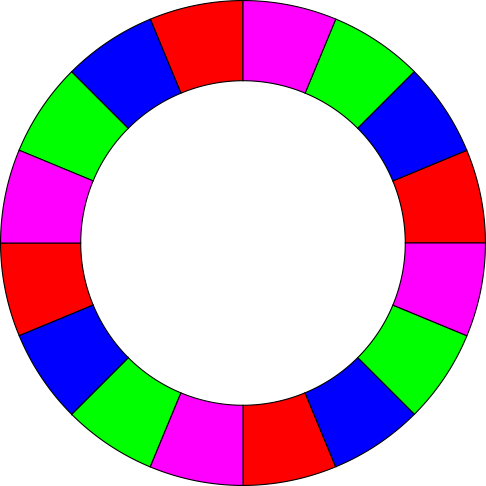
\includegraphics[width = 0.5 \textwidth]{_generated/pappus_exhaustion01.pdf}
\end{figure}

Since the cross-section has a vertical line of symmetry, if we take any piece and flip it to
rotate in the opposite direction, the ends of that piece can still be made to line-up with the
previous piece. Doing so, we can rearrange the pieces to "snake" back and forth. We use a number
of pieces that are a multiple of four, because this way the endpoints of the "snake" will be
aligned. See the figure below,

\begin{figure}[h]
\centering
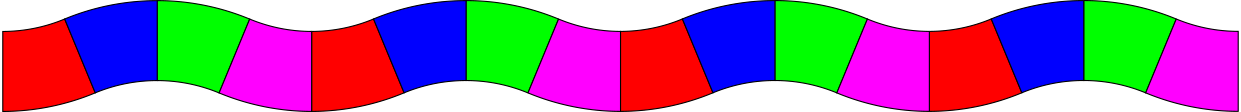
\includegraphics[width = 0.5 \textwidth]{_generated/pappus_exhaustion02.pdf}
\end{figure} 

Now, intuitively, as we make the number of pieces larger, the "snake" gets closer to a straight
cylinder. We see that each side of the cylinder is made of an equal number of pieces of arcs
coming from the "outer" circle of revolution as the "inner" circle of revolution. Let these
radii be \(r_1\) and \(r_2\). Then, intuitively we should have that sides of the cylinder are
\(2\pi(r_1 + r_2)/2\).

Let us prove this more rigorously.

Now, for each arc coming from the outer radius \(r_2\), from elementary geometry we have that the
width of the arc (NOT the length) is exactly
\begin{equation}
w_{\text{piece}} = 2r_2\sin\left(\frac{\pi}{4n}\right).
\end{equation}
Similarly for \(r_1\).

So we get that the total width of the snake is
\begin{equation}
w_n = 4n r_1 \sin\left(\frac{\pi}{4n}\right) + 4n r_2 \sin\left(\frac{\pi}{4n}\right).
\end{equation}
So \(w_n \to \pi r_1 + \pi r_2\). This is equal to the circumference of the circle formed by the
centroid of the cross-section (the symmetry of the cross-section gives us that the centroid has
radius \((r_1 + r_2)/2\)).

Technically, this last limit used that \(\frac{\sin(\theta)}{\theta} \to 1\) as \(\theta \to 0\).
This doesn't need to the full force of calculus to be shown as it follows from the classical
argument of comparing areas of triangles to areas of circular regions.

Now, we need lower and upper bounds on the volume of each rearrangement depending on \(n\). Look
at four consecutive segments of the "snake" and project their faces onto the plane of the base of
the "snake". We can use the areas of the intersections and the unions of these projections to give
us lower and upper bounds on the volume of the "snake" (which is equal to the volume of the
revolution). This is due to the face that snake is between the cylinder formed by the intersection
of the proejections and the cylinder formed by the union of the projections.

See the figures below for the pictures of the intersections and unions of the projections.
\begin{figure}[h]
\centering
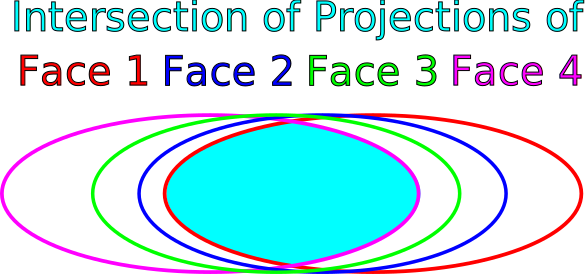
\includegraphics[width = 0.7 \textwidth]{_generated/pappus_intersection.pdf}
\end{figure}

\begin{figure}[h]
\centering
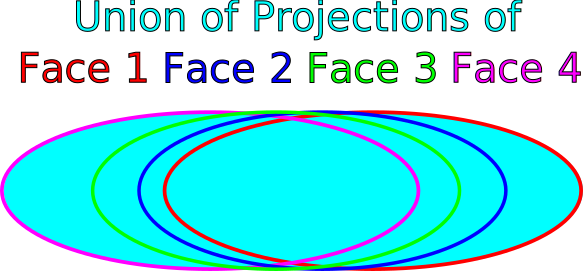
\includegraphics[width = 0.7 \textwidth]{_generated/pappus_union.pdf}
\end{figure}

Let the area of the intersection be \(I_n\) and the area of the union by \(U_n\). So we see that
the volume \(V\) of the body of revolution is bounded by
\begin{equation}
I_n w_n \leq V \leq U_n w_n.
\end{equation}

How it should be clear that are the number of pieces gets larger, the areas \(I_n\) and \(U_n\) get
closer to the area of the original cross section \(A\). Furthermore, we already showed that
\(w_n \to 2\pi r_{\text{centroid}}\). So from the pinching theorem, we get that
\begin{equation}
V = 2\pi r_{\text{centroid}} A.
\end{equation} 
